\section{Empirical comparison of KL objectives}

% Section~\ref{sec:estep_sleep_compare} motivates the wake-sleep approach by comparing variational posteriors obtained by optimizing the ELBO against those obtained by optimizing the sleep objective.
% Then, StarNet is tested on blended simulated stars in Section~\ref{sec:deblending_test}.
% Finally, in Section~\ref{sec:results_on_m2}, StarNet is employed to catalog the SDSS image of the M2 globular cluster. The StarNet catalog is compared with existing cataloging methods.

\label{sec:elbo_sleep_compare}

A simple example demonstrates that there exist shallow local optima in the ELBO
where the fitted approximate posterior is far in KL divergence from the exact posterior.
These local optima result in unreliable catalogs.
The expected forward KL, by taking advantage of complete data, appears to have a more favorable optimization landscape.
The simulated $20\times20$ single-band image $x_{test}$ is shown in Figure~\ref{fig:optim_path}(d).

We compare three approaches to deblending. The first two approaches directly optimize the ELBO,
\begin{align}
\mathcal{L}_{elbo}(\eta; x) = \Expect_{q_{\eta}(z \mid x)}\Big[\log p(x, z) - \log q_{\eta}(z \mid x)\Big],
\label{eq:elbo_on_test}
\end{align}
evaluated at $x = x_{test}$. 
The third approach minimizes the expected forward KL~\eqref{eq:sleep_obj}.
In each case, $q_\eta$ is the inference network from Section~\ref{sec:nn_architecture}.
The input to the network is a $10\times 10$ tile with no padding.

Note that the expected forward KL does not depend on $x_{test}$.
Optimizing $\mathcal{L}_{fwd}$ only requires sampling catalogs from the prior
and simulating images conditional on each catalog.
The prior on the number of stars was set to Poisson with mean $\mu = 4$.

Figure~\ref{fig:optim_path}~(top row) charts the test ELBO~\eqref{eq:elbo_on_test}
as optimization proceeds in our three approaches.
The first approach optimizes the ELBO with SGD and a REINFORCE plus control-variate gradient estimator~\citep{ranganath2013black}.
The path of the ELBO objective in this first approach is irregular, likely due to the high variance of the REINFORCE gradient estimator, 
and the optimization does not appear to converge (Figure~\ref{fig:optim_path}a).
For a lower-variance gradient estimator, the second approach employed the reparameterized gradient. To employ this gradient estimator, we analytically integrated the ELBO with respect to the number of stars $N$ to remove the discrete random variable.
See Appendix~\ref{sec:reparam_details} for details about the gradient estimators.
Using reparameterized gradients instead of REINFORCE gradients enabled the optimization to converge to stationary points (Figure~\ref{fig:optim_path}b).
However, for two randomly initialized restarts,
the optimization found local optima where the negative ELBO is notably higher than other restarts.

These shallow local optima in the ELBO result in unreliable catalogs.
The bottom row of Figure~\ref{fig:optim_path} displays the estimated locations, defined as the mode of the fitted variational distribution.
Figure~\ref{fig:optim_path}(e) shows these locations after converging to a shallow local optimum.
Here, the upper left tile was correctly estimated to have two stars, but both estimated stars were incorrectly placed at the same location.
(One of the locations should be placed on the second star.)
To move one of the estimated locations to the second star, the optimization path must traverse a region where the log-likelihood is lower than the current configuration (Figure~\ref{fig:local_optima_cartoon}).
The displayed configuration is a local optimum where the gradient with respect to its locations is approximately zero.

On the other hand, using
the expected forward KL does not directly optimize the test ELBO.
However, the test ELBO increases nonetheless, because the variational posterior
better approximates the exact posterior as the optimization proceeds.
Optimizing $\mathcal{L}_{fwd}$ consistently converged to
a similar ELBO across all restarts and avoided shallow local optima (Figure~\ref{fig:optim_path}c).
At each iteration of SGD, 
the evaluated loss is quadratic in 
the logit-location estimate
$\mu_\ell$ (\ref{eq:gaussian_sleep_loss}),
and the gradient does not vanish.
By avoiding shallow local optima, the variational distribution fit with the forward KL
always placed its mode on the four true stars in our trials.
An example of successful detection by fitting with
$\mathcal{L}_{fwd}$ is shown in~Figure~\ref{fig:optim_path}(f).

\begin{figure}[!htb]
    \centering
    \begin{subfigure}[t]{0.9\textwidth}
    \centering
    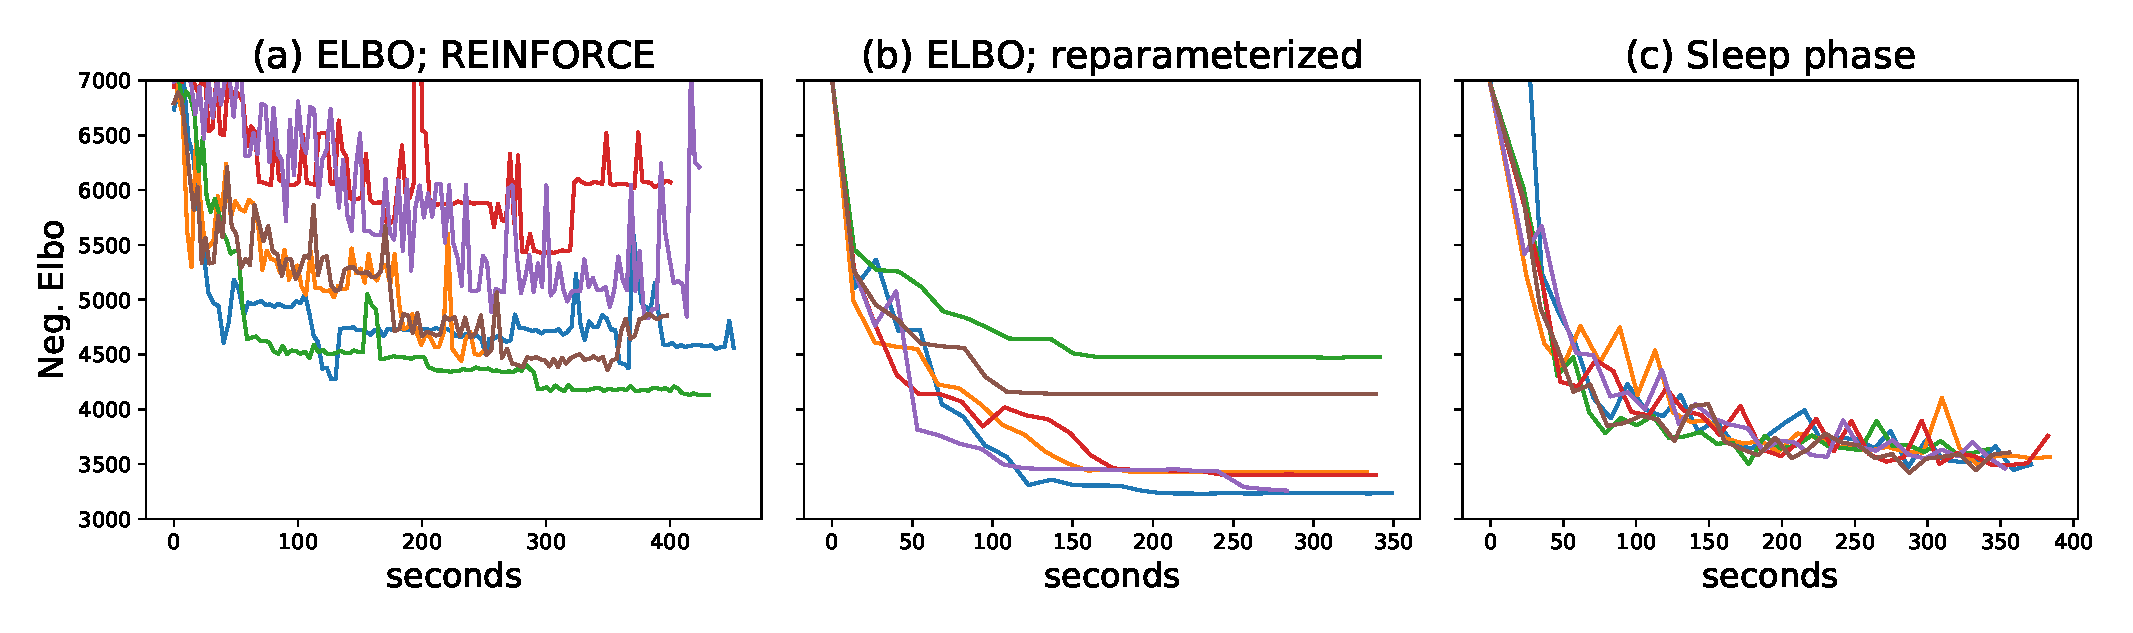
\includegraphics[width=\textwidth]{figures_vg/elbo_vs_sleep/optim_path_compare.eps}
    \end{subfigure}
    \begin{subfigure}[t]{\textwidth}
    \centering
    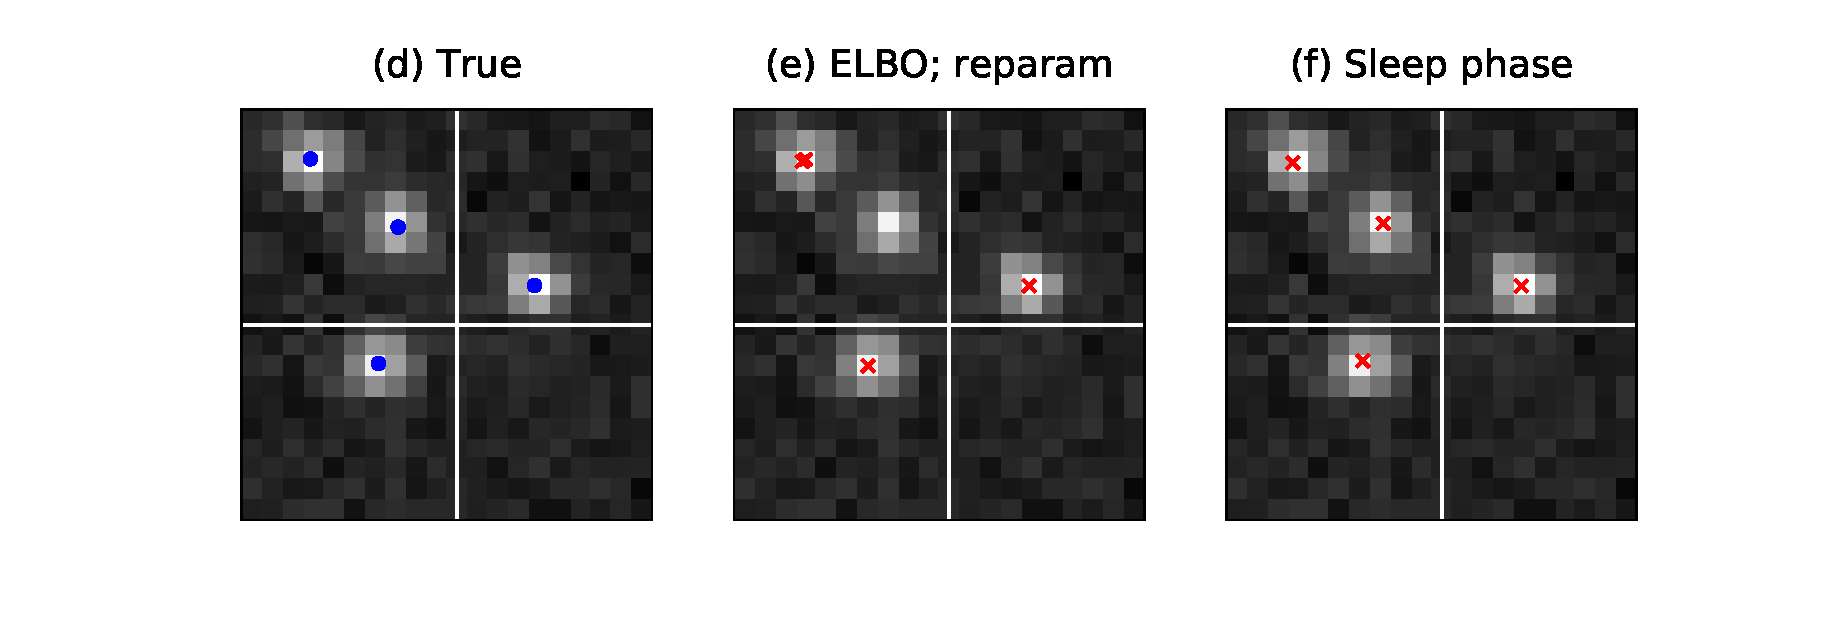
\includegraphics[width=0.9\textwidth]{figures_vg/elbo_vs_sleep/optim_path_detect_compare.eps}
    \end{subfigure}
%    \vspace{-1cm}
    \caption{(Top row) The negative ELBO as the optimization progresses for six random restarts.
    (Bottom row) In red, modal locations from ELBO-optimized and $\mathcal{L}_{fwd}$-optimized variational posteriors, for one of the six restarts.
    In blue, the true locations. }
    \label{fig:optim_path}
\end{figure}

% Figure~\ref{fig:gradzero_cartoon} shows a schematic of the optimization landscape as a function of locations.
% Recall that locations are parameterized between 0 and 1, and the neural network returns a variational mean parameter $\mu_\ell$ for the logit-location.
% When $\mu_\ell$ is far from the correct location (in logit space), the gradient of the ELBO with respect to $\mu_\ell$ vanishes.
% To see this, observe that the PSF is nearly zero everywhere except for a few pixels around its center. Therefore, a small shift in estimated location $\mu_\ell$ does not significantly change the likelihood unless the estimated location is within a ``PSF radius" of the correct location.
% On the other hand, the sleep objective is quadratic in the logit-location estimate $\mu_\ell$ (see Equation~\ref{eq:gaussian_sleep_loss}).
% Thus, the further the estimated location is from the correct location (in logit space), the larger the gradient. The gradient does not vanish in the sleep objective.

\begin{figure}[!htb]
    \centering
    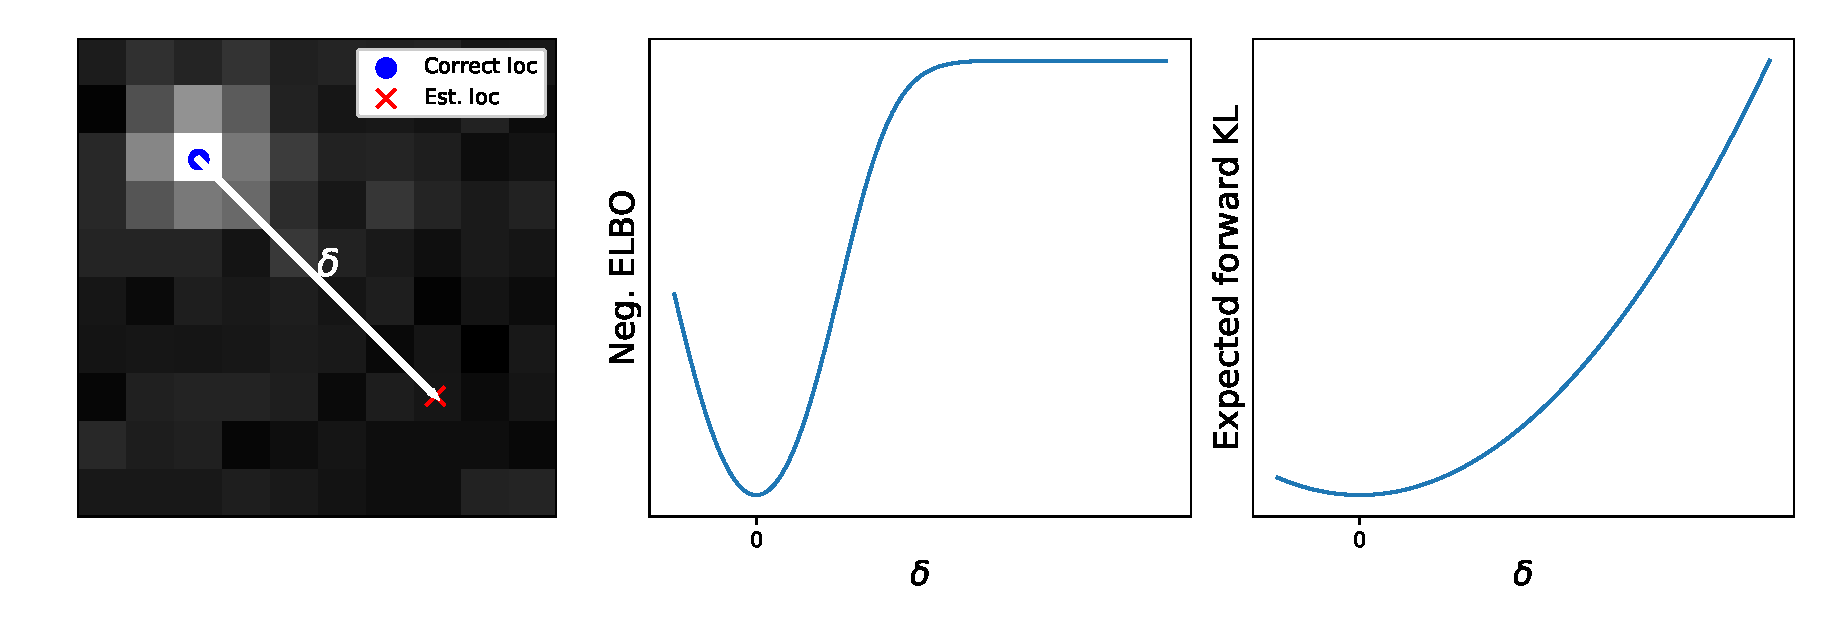
\includegraphics[width=0.9\textwidth]{figures_vg/elbo_vs_sleep/local_minima_cartoon.eps}
%    \vspace{-0.5cm}
    \caption{An illustration of local optima in the ELBO objective.
    To move an estimated location to a correct location,
    the optimization path must traverse a region where the negative ELBO is larger than the current configuration.
    In contrast, when optimizing the expected forward KL with SGD, each iteration evaluates a
    quadratic loss between a true and estimated location,
    and the gradient does not vanish. }
    \label{fig:local_optima_cartoon}
\end{figure}

Finally, note that low-variance gradients of the ELBO for this simple example were constructed by analytically integrating out $N$, 
and this was only possible because the image consisted of only four tiles. 
For each tile, the variational distribution has support over only 0, 1, or 2 stars.
Since the variational distribution factorizes over the four tiles, integrating $N$ is a summation of $3^4 = 81$ terms.
On larger images with more tiles, analytically integrating $N$ would be computationally infeasible,
and the standard reparameterization trick would not apply as it does in this small illustrative example.

% On a larger images where $N$ is on the order of $\sim1000$ (e.g. on M2), analytically integrating out $N$ would be infeasible.

% Only then could the reparameterization trick be applied to the ELBO, as the remaining latent variables are continuous.

% In this example, the variational distribution has support over only 0, 1, or 2 stars for each tile.
% Since the variational distribution factorizes over the four tiles, integrating $N$ is a summation of $3^4 = 81$ terms.
% On larger images with more tiles, analytically integrating $N$ would be computationally infeasible,
% and the simple reparameterization trick would not apply as it does in this small illustrative example.

% Figure~\ref{fig:sim_data100x100} displays our results on a larger example: a simulated $100\times 100$ pixel image with fifty stars.
% The tiles again consisted of $10\times 10$ pixel regions.
% Optimizing the ELBO does not produce accurate location estimates and appears to be hindered by regions with little gradient information; optimizing the sleep objective produced much improved location estimates.


% \begin{figure}[!htb]
%     \centering
%     \begin{subfigure}[!t]{0.59\textwidth}
%     \centering
%     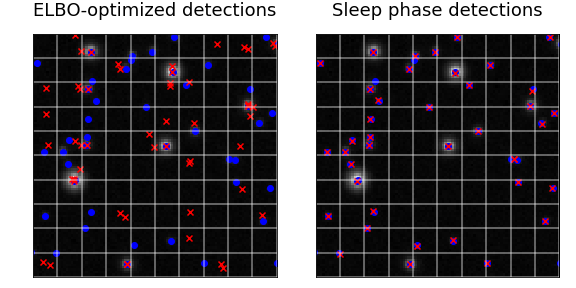
\includegraphics[width=\textwidth]{figures/elbo_vs_sleep/optim_path_detect_compare_100x100.png}
%     \end{subfigure}
%     \begin{subfigure}[!t]{0.4\textwidth}
%     \centering
%     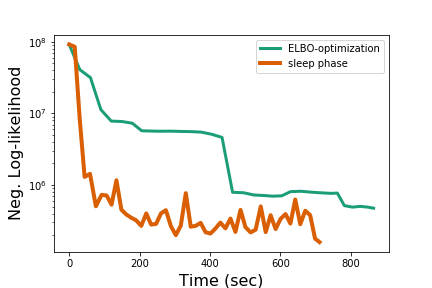
\includegraphics[width=\textwidth]{figures/elbo_vs_sleep/optim_path_compare_100x100.png}
%     \end{subfigure}
%     \caption{
%     (Left) Detections produced by ELBO optimization on a $100\times 100$ pixel test image.
%     Correct locations are blue and estimated locations are red.
%     (Middle) Detections produced by the sleep phase optimization.
%     (Right) The negative conditional log-likelihoood, $-\log p(x|\hat z)$, where $\hat z$ is the mode of the variational posterior and $x$ the
%     $100\times 100$ pixel test image. }
%     \label{fig:sim_data100x100}
% \end{figure}
